%book template given by EG Goodaire: http://www.math.mun.ca/~edgar/thesis.html --Thanks!
\documentclass[11pt]{book} 
\usepackage{amsmath} %Never write a paper without using amsmath for its many new commands 
\usepackage{amssymb} %Some extra symbols 
%\usepackage{makeidx} %If you want to generate an index, automatically 
\usepackage{graphicx,caption} %If you want to include postscript graphics 
\usepackage{mystyle} %Create your own file, mystyle.sty where you put all your own \newcommand statements, for example. 

%\includeonly{chaptr2} %If you just want to process chaptr2.tex 


\begin{document} 

%inspired by http://en.wikibooks.org/wiki/LaTeX/Title_Creation#A_practical_example
\begin{titlepage}
\begin{center}

% Upper part of the page. The '~' is needed because \\
% only works if a paragraph has started.
\noindent\begin{minipage}{.4\textwidth}
\centering

\includegraphics[width=\linewidth]{./img/uva-logo.png}~\\[.5cm]
\textsc{\normalsize University of Virginia}\\[1.5cm]
\end{minipage}
\hfill
\noindent\begin{minipage}{.4\textwidth}
\centering

\includegraphics[width=\linewidth]{./img/duke-logo.png}~\\[.5cm]
\textsc{\normalsize Duke University}\\[1.5cm]
\end{minipage}
\\[80pt]
\textsc{\Large HiFrost Reference Manual}\\[0.5cm]

% Title
\HRule \\[0.4cm]
{ \huge \bfseries The HI$\gamma$S Frozen Spin Target \\[0.4cm] }

\HRule \\[1.5cm]

% Author and supervisor
\begin{minipage}{0.4\textwidth}
\begin{flushleft} \large
\emph{Author:}\\
Ryan \textsc{Duve}
\end{flushleft}
\end{minipage}
\begin{minipage}{0.4\textwidth}
\begin{flushright} \large
\emph{Supervisor:} \\
Blaine \textsc{Norum}
\end{flushright}
\end{minipage}

\vfill

% Bottom of the page
{\large \today}

\end{center}
\end{titlepage}
\pagestyle{empty} %no page numbers on first pages
\chapter*{Preface}
\thispagestyle{empty} 


HiFrost is nuclear polarized target apparatus consisting of a dilution refrigerator, internal magnetic coil, microwave guide and NMR coil.  External components of HiFrost include a polarizing magnet, microwave generating EIO, pump and vacuum system to run the dilution refrigerator, and the Q-Meter/Yale Card set up for running the NMR. 


To polarize a target, chemically doped or irradiated beads are placed in the inner-most chamber, the fridge is assembled around the beads and the whole fridge is swung to align with the HIGS gamma beam.  The beads are cooled with liquid helium and polarized with a large external magnet, with an EIO providing microwaves necessary for dynamic nuclear polarization.


To achieve frozen spin mode, the internal magnet is ramped on as the external magnet is ramped off, so eventually the external magnet can be powered down and removed while keeping the polarized beads in a steady magnetic field. 
\frontmatter 
\tableofcontents 

\mainmatter 
\chapter{History} 
\label{history} % So I can \ref{altrings} later. 

\section{Polarized Targets}

\section{Inception}  
 
\section{CERN} 
 
\section{Geesthacht} 

\section{Virginia}

\section{Duke}
\chapter{Theory of Operation} 
\label{theory}  
\section{Nuclear Polarization}
In the presence of a magnetic field, spin-\half{} nuclei tend to align themselves along the axis of the field.  The polarization of the ensemble of particles is defined by 

$$P=\frac{\uparrow-\downarrow}{\uparrow+\downarrow},$$

where ($\downarrow$, $\uparrow$) is the population of nuclei with $m_z$=(-\half,\half).

\subsection{Thermal Polarization Derivation}

 \subsection{DNP}
Dynamic Nuclear Polarization (DNP) is a process of using microwave radiation to pump electron-proton pairs to higher energy (polarized) states.  The relaxation time for the electron is much shorter than that of the proton, so the proton remains polarized while the electron is able to be paired with other protons for polarization.

\begin{figure}
 \centering
 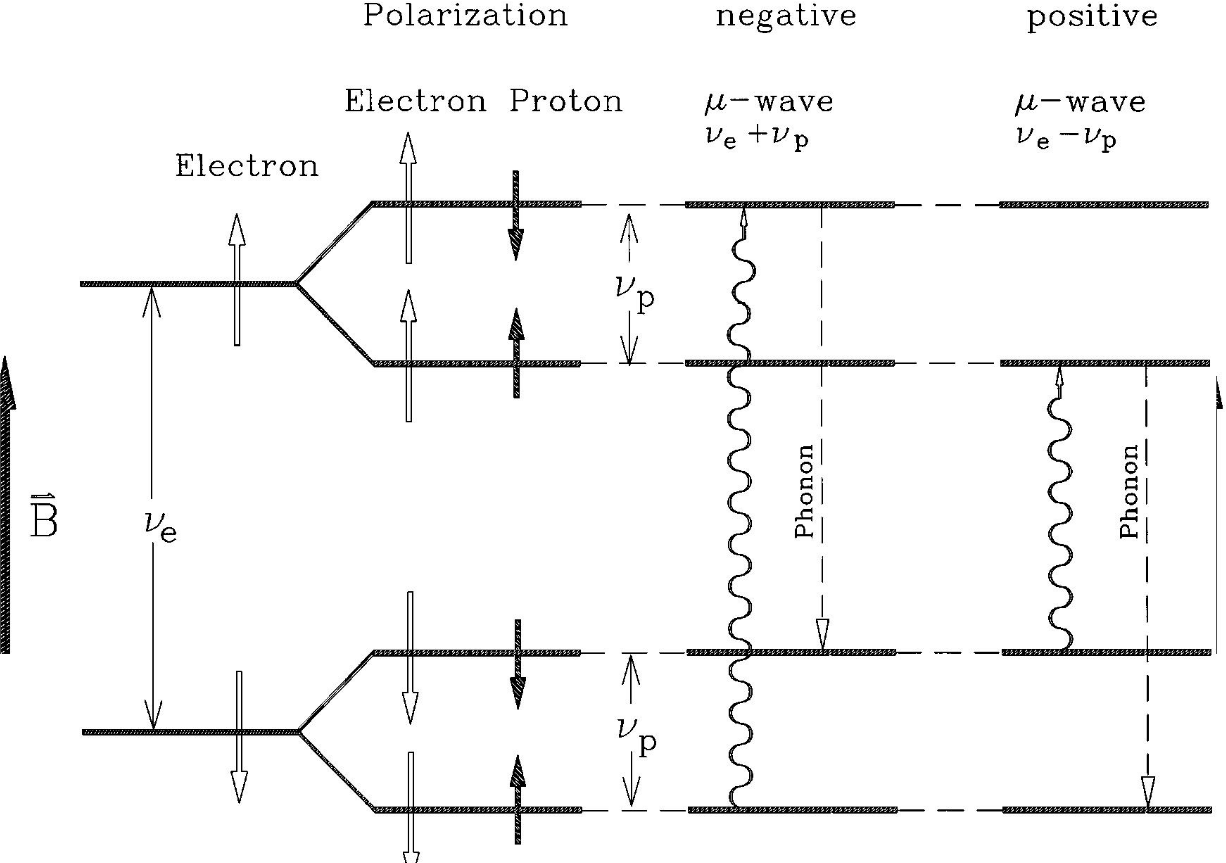
\includegraphics[scale=.25]{img/dnp.png}
 % dnp.png: 1226x863 pixel, 72dpi, 43.25x30.44 cm, bb=0 0 1226 863
 \caption{DNP diagram \cite{dnpdiagram}.  The white arrows are electron polarization and the black arrows are proton polarization.  Microwaves at a frequency difference $\nu_e\pm\nu_p$ flip the spins of both particles, and the electron's superior lattice coupling ensures it will flip back before the proton.}
 \label{fig:dnp-diagram}
\end{figure}


The microwave frequency can either be the sum of the proton and electron splitting frequency or the difference, depending on whether the nucleons are to be aligned with or against the magnetic field. 
\section{NMR}

Nuclear Magnetic Resonance (NMR) is the method we use to measure the polarization of the target material.  Essentially, a coil in the immediate vicinity of the target acts as the inductor in an LCR circuit, the inductance of which changes as a function of the magnetic susceptibility of the nuclei in the coil.  Since the magnetic susceptibility and polarization are related, the resonance frequency of the LCR circuit tell us information about the polarization of the target material\cite{qmeterbook}. 

\subsection{Liverpool Q-Meter}

\subsubsection{$\lambda$/2 Cable}

\subsubsection{Diode Detector}

\subsubsection{Phase Sensitive Detector and BRM}

\subsection{PDP}

\section{Frozen Spin} 
 
 The target is polarized in a 2.5 T field, called the polarizing field.  The target will lose all polarization in an environment free of magnetic field.  However, the detector cannot fit around the polarizing magnet, and the polarizing magnet would obstruct outcoming neutrons, anway).  To maintain polarization while the target is in the detector, an internal 0.5 T field is turned on inside the fridge and the polarizing magnetic is wound down and removed.  The 0.5 field, called the holding field, sufficiently maintains polarization of nucleons while the detector is moved aroud the target and data is taken.

\section{Refrigerator} 
Since the polarization goes like the inverse of temperature, colder environments make for better polarized targets.  In our case, we use a dilution refrigerator, one that mixes the two isotopes \het{} and \hef{} for cooling, to reach target temperatures below 0.1 K.

\subsection{\hef{}Cooling (Evaporator and Separator)}

\subsection{Dilution}

The dilution refrigerator principle relies on the splitting of a \het/\hef{} mixture into two distinct phases, a \het{} concentrated phase and a \het{} dilute phase.  The area labeled ``Two-phase region'' in Figure \ref{fig:dilutiondiagram} illustrates which mixtures, characterized by \het{} concentration, are inaccessible at which temperatures.  Since two distinct phases in thermal contact are always in or striving for thermodynamic equilibrium, changing the concentration of the dilute phase (by pumping \het{} out of it) will cause atoms from the concentrated phase to cross the phase boundary to restore balance.  Since the heat change of mixing (enthalpy difference between the dilute phase and concentrated phase) is positive, the \het{} crossing the phase boundary must absorb energy from the surrounding environment, which it does in the form of heat.\cite{hocktechniques}

\begin{figure}
 \centering
 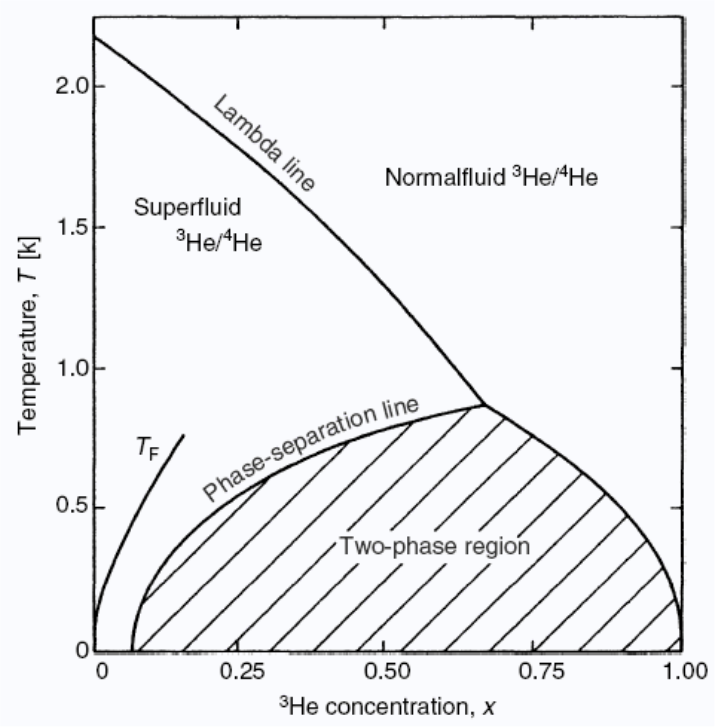
\includegraphics[scale=.45]{img/dilutiondiagram.png}
 % dilutiondiagram.png: 715x727 pixel, 72dpi, 25.22x25.64 cm, bb=0 0 715 727
 \caption{The famous diagram that shows the splitting of two distinct phases of $\het$-$\hef$ mixture. \cite{dilutiondiagram}}
 \label{fig:dilutiondiagram}
\end{figure}
 



\chapter{Hardware}
\label{hardware}
This chapter is an index and a catalog of all the equipment used in the project.
 
\section{Fridge}
  \subsection{Assembly Tools}
\subsubsection{OVC}

\begin{itemize}
  \item wire gripping pliers
  \item 5 mm allen key
  \item tee pilot pins  
\end{itemize}

\subsubsection{IVC}
\begin{itemize}
  \item solder station
  \item 2.5 mm allen key
  \item indium waste box
  \item wooden or hard plastic q-tips
  \item wire cutting pliers
  \item isopropyl alcohol 
\end{itemize}

\subsubsection{Microwave guide support}

\begin{itemize}
  \item flat head screwdriver
  \item fine tip squeeze-to-open tweezers 
\end{itemize}
 
\subsubsection{Mixing chamber}

\begin{itemize}
  \item mixing chamber customized open wrench
  \item 1.5 mm allen key
  \item indium waste box
  \item wooden or hard plastic q-tips
  \item wire cutting pliers
  \item isopropyl alcohol 
\end{itemize}


  \subsection{Cryogenic Instruments}

\subsubsection{\hef{} sensors}
  \begin{itemize}
   \item 2x \textit{Lake Shore\circledR} DT-670 silicon diode
\item \textit{Lake Shore\circledR} PT-102 platinum RTD
\item \textit{Lake Shore\circledR} Quad-Lead cryogenic wire, 36 AWG
  \end{itemize}
\subsubsection{\het{} sensors}
\begin{itemize}
 \item \textit{Lake Shore\circledR} DT-670 silicon diode
 \item \textit{Omega\circledR} KHLV-0502 Kapton heater
 \item \textit{Lake Shore\circledR} RX-202A-AA ruthenium oxide sensor
 \item \textit{Lake Shore\circledR} GR-200A-30 germanium diode
 \item 4-wire Matsushita resistor (model unknown) 

\end{itemize}

  \subsection{Magnet Leads}
\begin{itemize}
 \item OFHC copper leads
\item insulating mylar
\item Kapton tape
\item small flat head screwdriver
\item minature flat head screws
\item \textit{Solid Sealing\circledR} KT20678 copper conductor KF feedthrough
\end{itemize}


\section{Target Material}
\begin{itemize}
 \item cryogenic storage \lnn{} dewar
\item open styrofoam tub, about 5-10 liters
\item tweezers
\item hemostats
\item \lnn{} transfer dewar
\item cryogenic gloves
\end{itemize}

\section{Fridge Stand Mounting/Swinging Tools}

\begin{itemize}
  \item 13 mm combination wrench
  \item long-shaft 3/16\inches{} ball driver
  \item 10 mm combination wrench
  \item 5 mm allen key
  \item fridge lever
  \item \textit{80/20$^\circledR$} 5/16\inches{}-18 nuts, bolts
\end{itemize}


\section{Pump Station Area}
  \begin{itemize}
   \item Alcatel or VIC leak checker
   \item KF-25 plastic blank off
   \item KF-25 flexible hose
  \end{itemize}

  \subsection{\het{} Pumps} %use \hef{} to put space after newcommand
  \subsection{\hef{} Pumps}
  \subsection{\lnn{} Trap}
\begin{itemize}
 \item \lnn transfer dewar
\item cryogenic gloves
\item heat gun
\end{itemize}

  \subsection{Helium Gas Cylinders}

  
\section{Vault Pumps}
  \subsection{OVC}
  \subsection{IVC}

\section{Cryogenics}
  \subsection{Safety}
  \subsection{Transfer Lines}

\section{Vault Electronics Rack}
  \subsection{Patch Panel}
  \subsection{}

\section{NMR}

\section{Microwaves}
\chapter{Practical Operation} 
\label{chapter:practical-op}
\begin{figure}[!h]
 \centering
 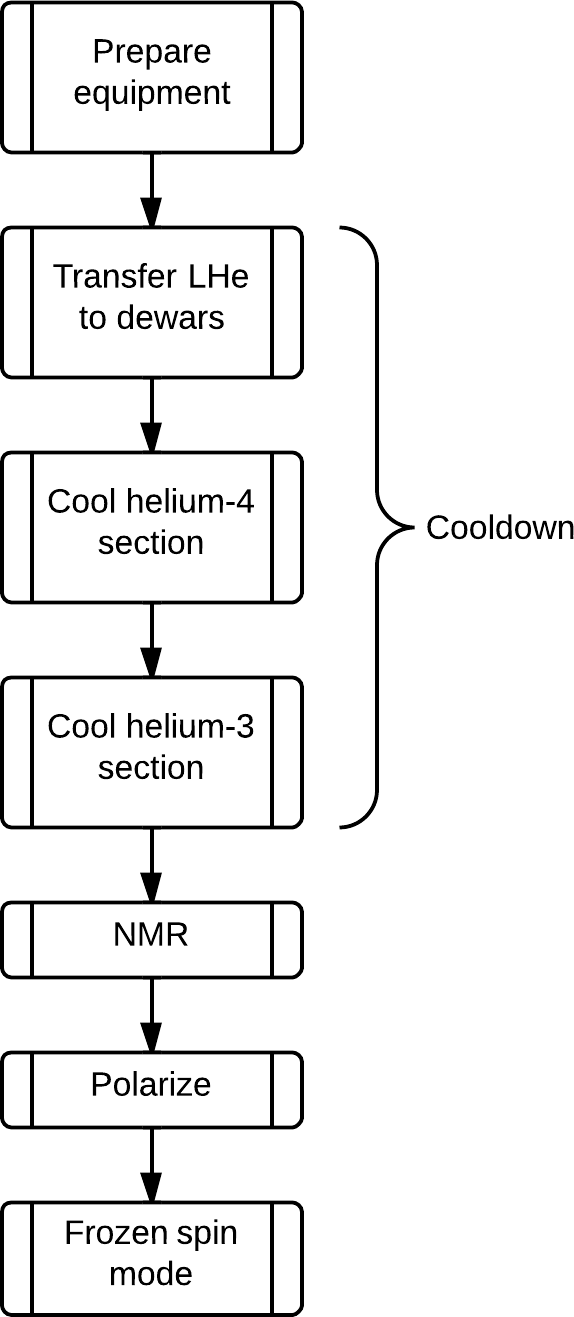
\includegraphics[scale=.24]{./img/cooldown-overview-flowchart.png}
 % cooldown-overview-flowchart.png: 102x490 pixel, 100dpi, 2.59x12.45 cm, bb=0 0 73 353
 \caption{Practical steps to polarize target material with HiFrost.}
 \label{fig:cooldown-overview-flowchart}
\end{figure}

This chapter assumes the reader is familiar with everything safety related.  Read Chapter \ref{safety} before attempting anything here.



\section{Cooldown}
\subsection{Prep}
\label{practical-op:prep}
Go down the checklist found in Appendix \ref{appendix:checklist-for-cooldown}, reporting any issues to the senior cooldown scientist.

\textbf{This step is not optional}: the rest of this operational procedure assumes all prep work is successfully completed and equipment bugs are worked out.  See walkthroughs for specifics tasks in Chapter \ref{procedures}.

\section{LHe Transfer Overview}

Figure \ref{fig:cryo-schematic-all} is a schematic of the LHe transfer system.  More detailed figures of the dewars are found later in the chapter, and complete technical drawings of the TLs are found in Appendix \ref{appendix:tl-drawings}.

\begin{figure}[htbp!]
 \centering
 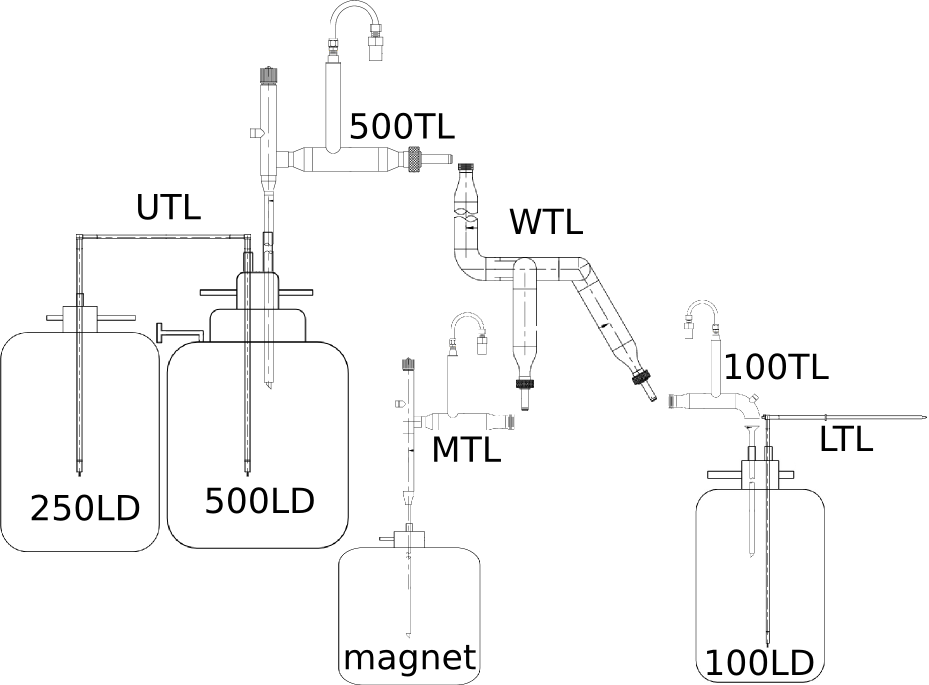
\includegraphics[width=\textwidth]{./img/cryo-schematic-all.png}
 % cryo-schematic-all.png: 0x0 pixel, 0dpi, 0.00x0.00 cm, bb=
 \caption{Schematic overview of the LHe transfer and storage system.}
 \label{fig:cryo-schematic-all}
\end{figure}


\subsection{Dewar Filling}
The 500LD and 100LD are initally filled before cooling the fridge.  The magnet is filled either before or after dilution.

The 250LD has an LHe outlet port, a pressurization/exhaust port and the pressure relief port, shown in Figure \ref{fig:250LD-cartoon}.  Each port has an accompanying valve.

The 500LD has an inlet port (for LHe filling and the level probe), an outlet port, a pressurization port, a vacuum pump out port and a pressure relief port, as shown in Figure \ref{fig:500LD-cartoon}.  Only the pressurization, vacuum pump out and pressure relief ports have accompanying valves.


\begin{figure}[!htbp]
\centering
 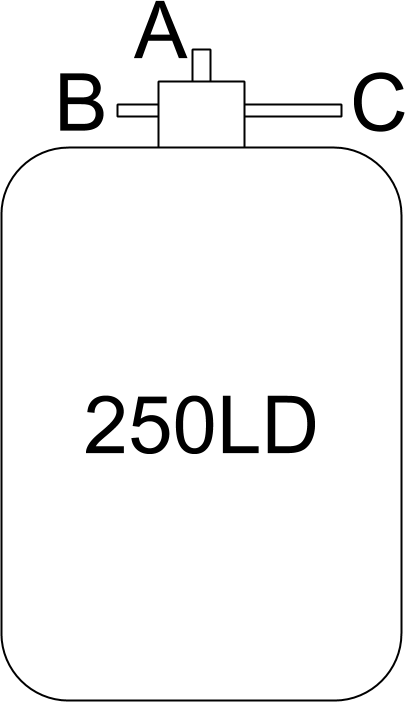
\includegraphics[width=.25\textwidth]{./img/250LD-cartoon.png}
 % 500LD-cartoon.pdf: 0x0 pixel, 0dpi, nanxnan cm, bb=
 \caption{An example of 250LD ports: A) LHe outlet port, B) pressure relief valve, C) pressurization/exhaust port.}
 \label{fig:250LD-cartoon}
\end{figure}


\begin{figure}[!htbp]
 \centering
 \begin{minipage}{.35\textwidth}
 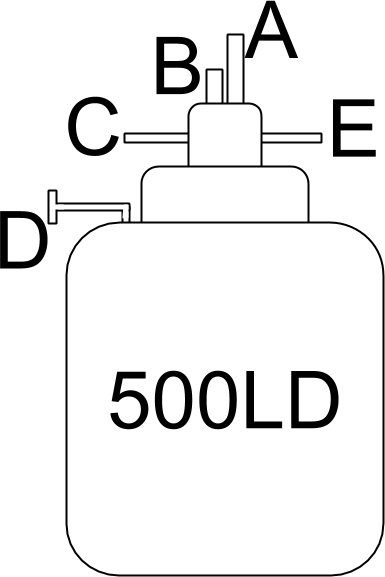
\includegraphics[width=\textwidth]{./img/500LD-cartoon.png}
 % 500LD-cartoon.pdf: 0x0 pixel, 0dpi, nanxnan cm, bb=
 \caption{The 500LD ports.}
 \label{fig:500LD-cartoon}
 \end{minipage}
 \quad
  \begin{minipage}{.50\textwidth}
 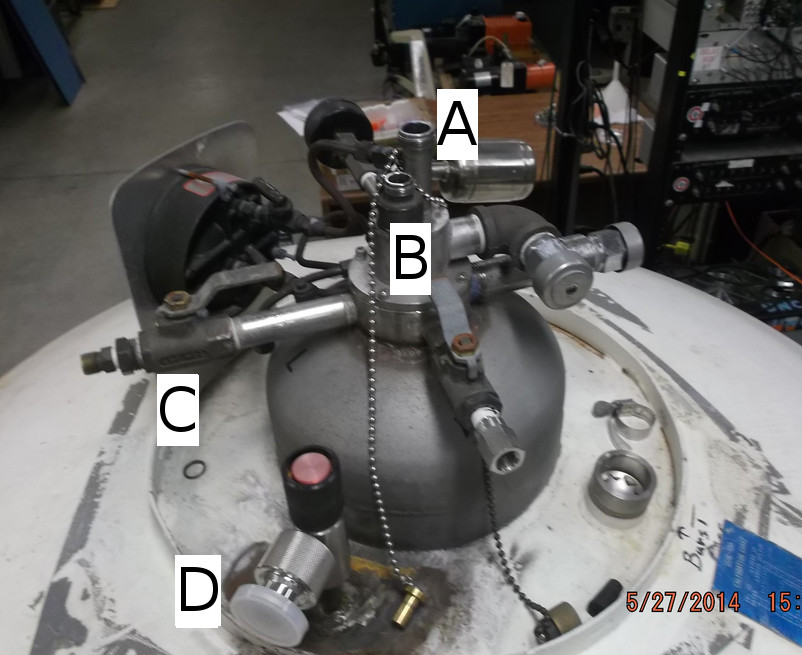
\includegraphics[width=\textwidth]{./img/500LD-photo.jpg}
 % 500LD-cartoon.pdf: 0x0 pixel, 0dpi, nanxnan cm, bb=
 \caption{Photo of 500LD: A) LHe inlet port, B) LHe outlet port, C) pressurization port, D) vacuum pump out port, E) pressure relief valve.}
 \label{fig:500LD-photo}
 \end{minipage}
 \end{figure}




\subsubsection{500LD Fill}
\label{practical-op:500LDfill}
\begin{enumerate}
 \item Weigh a full 250LD according to the procedure in Section \ref{weigh-250LD} before breaking the seal on it.
 \item Check 250LD level using the procedure in Section \ref{procedure:check-lhe-level}.
 \item Place correct Goddard fittings on the 250LD and/or the UTL.
 \item Blow out UTL with helium gas by fitting the universal hose over it and putting about 2 PSI on the helium cylinder. \label{procedure:500LDfill-blowoutUTL}
 \item $[$\textbf{initial 500LD fill only}$]$ Purge the 500LD with helium gas by hooking up the pressurization line, closing the main flow valve, opening the pressure release valve and putting 5 pounds of pressure on the 500LD for about 10 minutes (Figure \ref{fig:500LDfill-02-blow-out-500LD}).  Remove the pressurization line. \label{procedure:500LDfill-purge500LD}%for some godforsaken reason square brackets have to be in math mode to not ruin enumerated lists
 \item Open main flow valve on 500LD to vent pressure (if any), then open pressurization valve making sure the pressurization port is not pointed at anyone.
 \item Release the 250LD pressure from the main flow valve and close the pressure relief valve.  Slowly lower the correct end of the UTL down into the 250LD about 30 cm or until helium gas is blowing out the 500LD end, as shown in the left side of Figure \ref{fig:500LDfill-03-04-insert-UTL-in-250LD-and-500LD}.  Then, lower the 500LD end in as far as it can go, while continuing to slowly lower the 250LD side at a rate of about 2 cm/s.  A cold plume should be coming out of the 500LD.  Check that no gas is escaping through the Goddard fittings on either dewar (if it is, replace fitting o-rings). \label{procedure:insert-UTL-in-250LD}
 \item Hook up the pressurization line to the 250LD pressurization port using the procedure in Section \ref{procedure:attach-pressurization-line} and open the pressurization valve as shown in the right side of Figure \ref{fig:500LDfill-03-04-insert-UTL-in-250LD-and-500LD}.  There should now be 2 PSI on the 250LD. \label{procedure:insert-UTL-in-500LD}
 \item Periodically measure the 250LD level using the procedure in Section \ref{procedure:check-lhe-level}.  When it is empty, stop flow from the pressurization cylinder regulator and disconnect the pressurization line.
 \item Simultaneously raise both sides of the UTL out of the dewars and hang it on the wall to warm up.
 \item Bung the 500LD inlet port, close the 500LD pressurization valve, and leave open the pressure relief valve.
 \item On the 250LD, open the pressure release valve and close the main flow and pressurization valves.
 \item Recover the Goddard fittings from the 250LD and bring it back to the weigh area.  Record the final weight on the log sheet.
\end{enumerate}

\begin{figure}[htbp!]
 \centering
 \begin{minipage}{.47\textwidth}
 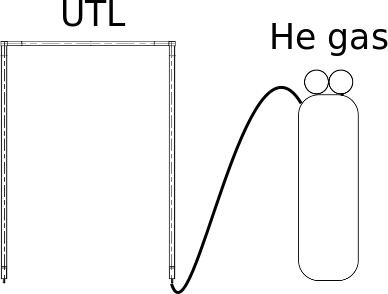
\includegraphics[width=\textwidth]{./img/500LDfill-01-blow-out-UTL.png}
 \caption{Blowing out the UTL with He gas (Step \ref{procedure:500LDfill-blowoutUTL}).}
 \label{fig:500LDfill-01-blow-out-UTL}
 \end{minipage}
 \quad
 \begin{minipage}{.47\textwidth}
 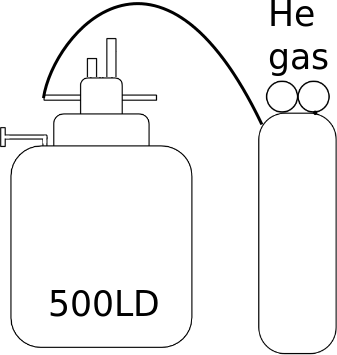
\includegraphics[width=\textwidth]{./img/500LDfill-02-blow-out-500LD.png}
 \caption{\textbf{Initial 500LD fill}, purging the 500LD with He gas (Step \ref{procedure:500LDfill-purge500LD}).}
 \label{fig:500LDfill-02-blow-out-500LD}
 \end{minipage}
\end{figure}

\begin{figure}[htbp!]
 \begin{minipage}{.38\textwidth}
 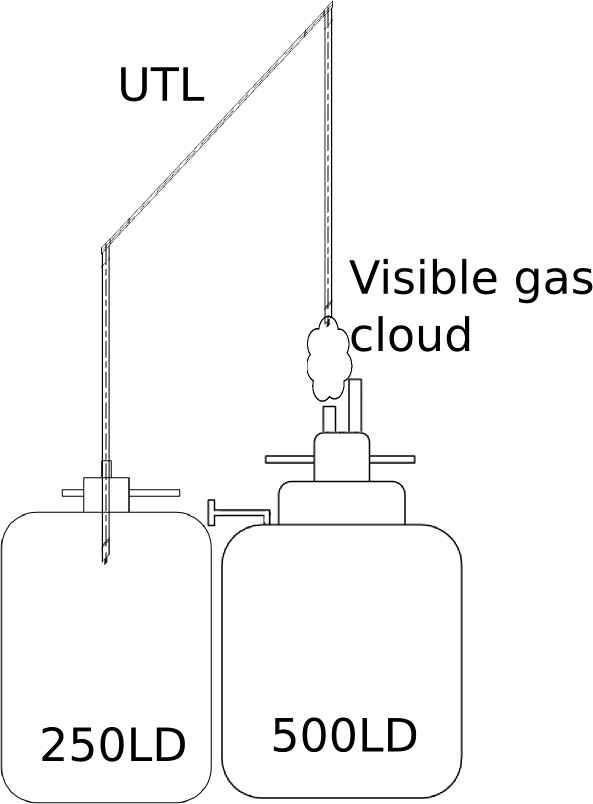
\includegraphics[width=\textwidth]{./img/500LDfill-03-insert-UTL-in-250LD.png}
 \end{minipage}
  \quad
 \begin{minipage}{.58\textwidth}
 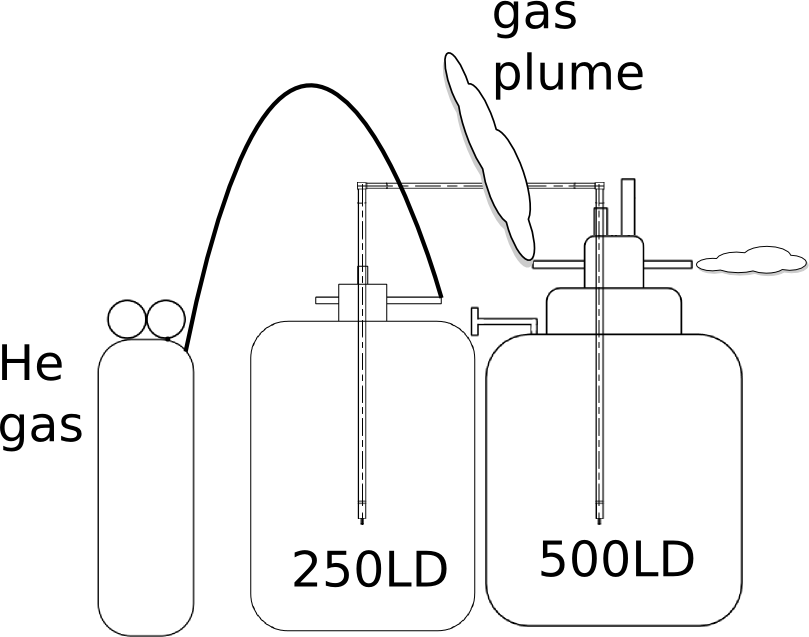
\includegraphics[width=\textwidth]{./img/500LDfill-04-insert-UTL-in-500LD.png}
 \end{minipage}
 \caption{Inserting the UTL first in the 250LD, then the 500LD, as described in Steps \ref{procedure:insert-UTL-in-250LD} and \ref{procedure:insert-UTL-in-500LD}.  The pressurization line is attached to the 250LD to facilitate liquid transfer.}
 \label{fig:500LDfill-03-04-insert-UTL-in-250LD-and-500LD}
 \end{figure}
 


\subsubsection{Initial 100LD Fill}

The 100LD has an entrance port, a main flow port, an exhaust port and a pressure relief port.  The exhaust and pressure relief ports have accompanying valves.
 
 \begin{figure}[!htbp]
 \centering
 \begin{minipage}{.55\textwidth}
 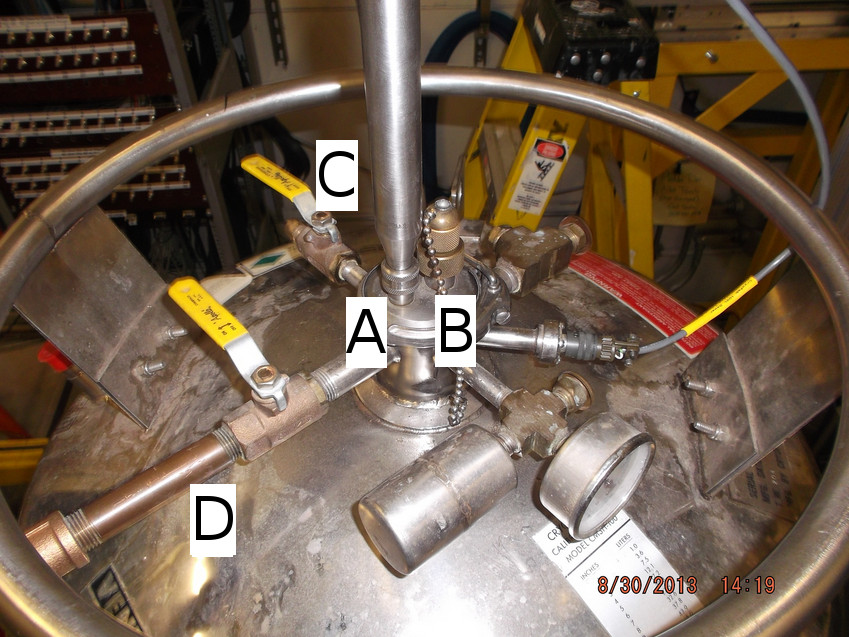
\includegraphics[width=\textwidth]{./img/100LD-photo.jpg}
 % 500LD-cartoon.pdf: 0x0 pixel, 0dpi, nanxnan cm, bb=
 \caption{Photo of 100LD: A) LHe inlet port, B) LHe outlet port, C) pressure relief valve, D) pressurization/exhaust port.}
 \label{fig:100LD-photo}
 \end{minipage}
 \quad
  \begin{minipage}{.40\textwidth}
 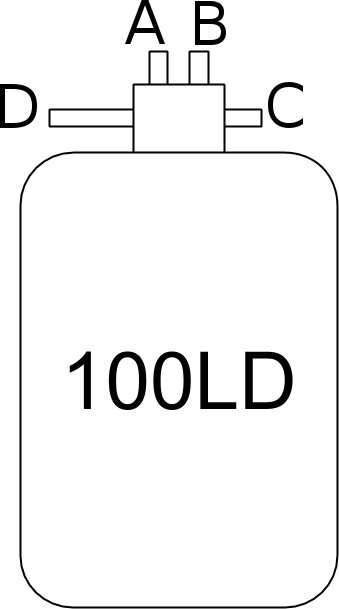
\includegraphics[width=\textwidth]{./img/100LD-cartoon.jpg}
 % 500LD-cartoon.pdf: 0x0 pixel, 0dpi, nanxnan cm, bb=
 \caption{100LD cartoon.}
 \label{fig:100LD-cartoon}
 \end{minipage}
 \quad
\end{figure}

\begin{enumerate}
 \item Purge the 500TL with helium gas.  Make sure the flow valve is open.
 \item Make sure the correct Goddard fittings are on the 500LD and/or 500TL.
 \item Install the 100TL in the 100LD and attach the bayonet to the WTL.
 \item Close the magnet LHe inlet valve on the WTL (blue valve).
 \item Open the 100LD exhaust valve, close the pressure release valve and bung the main flow valve.
 \item Remove the bung from the WTL by the pump station area.
 \item Hook up the helium gas line in the GV to the 100LD exhaust port and pressurize to 2 PSI.
 \item Verify there is a positive pressure on the WTL by the pump station.  Increase the helium cylinder pressure if necessary.  Wait 10 minutes for the 100LD, 100TL and WTL to purge.
 \item Close the 500TL flow valve and stop purging it.
 \item Vent the 500LD through the pressurization port.
 \item Open the 500LD main flow port.
 \item Close the 500LD pressurization and pressure relief valves.
 \item Slowly lower the 500TL about 30 cm until helium gas starts flowing out.  It may need to go further in first, depending on how full the 500LD is.
 \item Watch the gas plume coming out of the end of the 500TL.  Slowly lower the 500TL in the 500LD at a rate of 1cm/s until the plume looks like a blowtorch, then immediately insert into the WTL and tighten.
 \item \textbf{Immediately remove the pressurization line from the 100LD exhaust port and open the 100LD pressure relief valve.} Verify gas is coming out the exhaust and make sure the exhaust is pointing towards the center of the room and not at personnel (the plume will quickly grow).
 \item Slowly lower the 500TL all the way down into the 500LD and tighten the Goddard fitting.  Use the heat gun if the Goddard fitting freezes before the 500TL is completely in.
 \item Hook up the pressurization line to the 500LD pressurization port using the procedure in Section \ref{procedure:attach-pressurization-line} and open the 500LD pressurization valve.
 \item Turn on the 100LD level probe and watch the monitor for the level to increase.
 \item When the 100LD is full there will be a large white plume coming from the exhaust and the level probe will read around 24.9 (arbitrary units). Close the 500LD pressurization valve and remove the pressurization line.  Then vent the 500LD through the pressurization port and open the 500LD pressure relief valve.
 \item Close the 500TL flow valve.
 \item Close the 100LD exhaust valve.
\end{enumerate}

\subsubsection{100LD Fill During Run}

\begin{enumerate}
 
 \item Verify the 500LD is full enough to top off the 100LD.  If not see above 500LD fill procedure.
 \item Set the regulator on the helium pressurization cylinder to 2 PSI.
 \item Open the 100LD exhaust valve and make sure the exhaust port is safely facing the center of the room.
 \item Hook up the pressurization line to the 500LD pressurization port using the procedure in Section \ref{procedure:attach-pressurization-line}.
 \item Open the main flow valve on the 500TL, then close the 500LD pressure relief valve.
 \item Open the 500LD pressurization valve.
 \item Verify the 100LD Goddard Fittings are not leaking gas.  If they do, remove the pressurization from the 500LD and close the 500TL main flow valve immediately.  Consult a high ranking lab official.
 \item When the 100LD is full, remove the pressurization from the 500LD, open the 500LD pressure relief valve and close the 500TL main flow valve.
 
\end{enumerate}


\subsection{Cool \hef{} Section}

When the 100LD is full, the fridge has been backfilled with helium gas and the rest of the system is ready for a cooldown, the LTL is inserted into the 100LD and fridge.  The separator pumps on the fridge are started and the pressure difference is enough to pull helium from the 100LD (no dewar pressurization needed).

The LHe travels through the LTL into the separator, which collects liquid while rejecting gas.  The gas is pulled out through two lines, the ``separator'' line which precools the \het{} inlet, and the shield line which provides a heat shink for the radiation shield.

When the separator is full, control valve 1 (CV1) allows helium to flow to the evaporator and control valve 2 (CV2) directs LHe to the holding magnet and IVC can.  CV2 is also used to quickly cool the MC when target material is at risk of thermal damaged.

The evaporator can hold LHe at 4K, but evaporator pumps are run to lower the helium vapor pressure and lower the temperature down to a minimum of about 1K.

\subsubsection{Insert LTL}
\begin{enumerate}
 \item See Section \ref{practical-op:prep} to make sure the fridge is ready to take LHe.
 \item Check the 100LD level probe and top off if necessary (see directions above).
 \item Blow out LTL with helium gas.
 \item Make sure 100LD can roll out from under the fridge stand area (so the LTL can be inserted), back under the fridge stand area, and then up to the fridge.  The IVC pump cart may have to be shifted around.
 \item Put 4 PSI on the fridge via the following steps: adjust the helium gas regulator to 4 PSI, open the valves between the regulator and the separator manifold, close all other separator manifold valves (so gas does not flow to separator pumps).
 \item Remove the LHe inlet bung and KF clamp from the fridge and verify the positive pressure from the separator.
 \item Stop purging LTL with gas and place a rubber in the fridge side.
 \item Remove bung from 100LD main flow port and slowly insert the LTL until it lines up with the fridge.
 \item Roll the 100LD in place under the fridge stand.
 \item Remove the LTL bung and wait for the gas plume to look like a blue torch flame, then roll the 100LD towards the fridge until the LTL is fully inserted and tighten the KF clamp around the LTL-fridge inlet joint.
 \end{enumerate}
 
 \begin{enumerate}
 \item Open CV1 and CV2 about 2 turns each.
 \item Immediately turn off the pressurization from the helium cylinder and turn on the separator pumps.  Open all valves between the separator pumps and the fridge, including bypass valves.  Pump on shield at max flow for 30 minutes and separator for 15 minutes\cite{tapio-cooldown-procedure}.
 \item Separator flow is only kept high when there is no liquid in the separator yet; thereafter control the shield flow keeping it below 20 mmol/s and reduce the separator flow to 5 mmol/s (see Appendex \ref{appendix:slpm-conversion} for flow conversion). 
 \item TODO Cooldown diverges from June 2014 cooldown at this point; consider separate document
\end{enumerate}


\subsection{Cool \het{} Section}
\subsection{Dilution}

\section{Polarization}

\section{NMR}

\section{Frozen Spin}
\blindtext

\chapter{Procedures} 
\label{procedures}  
\section{Evacuating Transfer lines}

\subsection{Cryofab TLs}

\subsection{LTL}

\section{Indium Extrusion}

\section{Making/Breaking Indium Seals}

\section{Magnet Lead Installation}

\section{Mounting Fridge}

\section{Dismounting Fridge}

\section{Cleaning Viton/Buna O-rings}

\section{Changing Kenol Connectors}

\section{Installing Heating Tapes}

\section{Purging Helium Lines}

\section{Vacuum Rise Testing}

\section{Stripping Fridge}

\section{Assembling Fridge}

  \subsection{MC}
  \subsection{Microwave Guide Support}
  \subsection{IVC}
  \subsection{OVC}

\section{Removing/Replacing \het{} Baffles} 
%\include{chaptr3} 
%\include{chaptr4} 
%\include{chaptr5} 

\backmatter 
%\include{glossary} 
%\include{notat} 
%\bibliographystyle{amsalpha} %The style you want to use for references. 
%\bibliography{mr,refs} %The files containing all the articles and books you ever referenced. 
%\printindex %Make an index AUTOMATICALLY 

\end{document} ********End of master.tex 